\documentclass[12pt]{article}
\usepackage{multicol}
\usepackage{titlesec}
\usepackage{float}
\usepackage{graphicx}
\usepackage{amsmath}
\graphicspath{ {images/} }
\usepackage[paperheight=11in,paperwidth=8.5in,top=0.75in,bottom=0.75in,left=0.5in,right=0.5in,heightrounded]{geometry}
\pagestyle{empty}

\vspace{10mm}

\begin{document}
{
% Title and Authors
\centering \large \bf
KINEMATICALLY SIMILAR BASKETBALL FREE THROWS \break
HAVE SURPRISINGLY DIFFERENT MUSCLE CONTRACTION VELOCITY PROFILES\break
\\
\centering \normalsize \rm
Daniel A Hagen$^1$, *Steven Caja$^1$, *Suraj Chakravarthi$^2$, Francisco J Valero-Cuevas$^{1,3}$\break
\\
$^1$University of Southern California, Department of Biomedical Engineering, Los Angeles, CA, USA \break
$^2$University of Southern California, Department of Electrical Engineering, Los Angeles, CA, USA \break
$^3$University of Southern California, Department of Biokinesiology and Physical Therapy, Los Angeles, CA, USA \break
E-mail: dhagen@usc.edu Website: valerolab.org \break
*Equal Contributions\break
\\
}
\begin{multicols}{2}
\titleformat{\section}
  {\normalfont\fontsize{12}{15}\bfseries}{\thesection}{1em}{}
\section*{ABSTRACT}
The pursuit of the perfect basketball shot relies heavily on practice, with those capable of consistently accurate throws being paid millions of dollars as professional athletes. But why is it that practice or mimicry alone do not suffice to accomplish a professional level of accuracy? Recent work re-emphasizes that the neural control of limb movements is in fact overdetermined with the rotations of a few joints determining the length changes in all muscles [1, 2]. As pointed out by Sherrington [3], movement trajectories can be disrupted if even one muscle undergoing eccentric contraction fails to silence its stretch reflex appropriately. Thus throws requiring higher eccentric velocities require more accurate alpha-gamma co-activation control, and are thus more prone to variability. Additionally, higher concentric contraction velocities reduce muscle power output. Therefore, we investigated whether kinematically similar throws can exhibit large differences in eccentric and concentric muscle fiber contraction velocities [1].
\section*{METHODS}
The biomechanics involved in shooting a basketball are extremely complex. In order to make the modeling process more feasible, a few assumptions were made. First and foremost, the system was assumed to include only sagittal planar motion from the shoulder down with the angle of pronation fixed to 180$^{\circ}$. This was considered to be a fair assumption as our interest focused on the mechanics of a generalized free throw attempt with an emphasis on the fiber velocities of pertinent upper limb muscles. Here we assumed that the muscles that contributed to forearm pronation/supination and lateral shoulder abduction/adduction did not contribute to the generalized throw attempt. Second, we modeled the basketball shot as a simple ballistics equation, relating initial position and velocity (i.e. the point of release) to the desired endpoint (i.e. basketball net). \linebreak
We considered each shot to undergo three phases: the upstroke, the power stroke, and the follow-through. The upstroke was defined as the initial phase of the shot when the ball is brought from rest at the initial position upwards towards the cocked position (when the angular velocity about the elbow joint is zero). The power stroke was considered to be the phase of the shot immediately following the change in the direction of elbow rotation. And the follow-through was defined as the segment of the shot after the endpoint (distal portion of the hand) had reached its desired velocity (determined through kinematics of the ballistics equation) when the wrist flexes and the resulting endpoint force production generates "backspin" on the ball. To simplify the inverse kinematics, we assumed that the desired initial velocity of the projectile would be generated during the power stroke phase of the shot, thereby neglecting the follow-through and the resulting "backspin" rotation. Therefore, the final endpoint velocity of the hand and the end of the power stroke should have the initial projectile velocity of the ball required for a successful free throw attempt. Additionally, we have neglected air resistance and volumetric contractions
\end{multicols}
\begin{figure}[H]
\centering
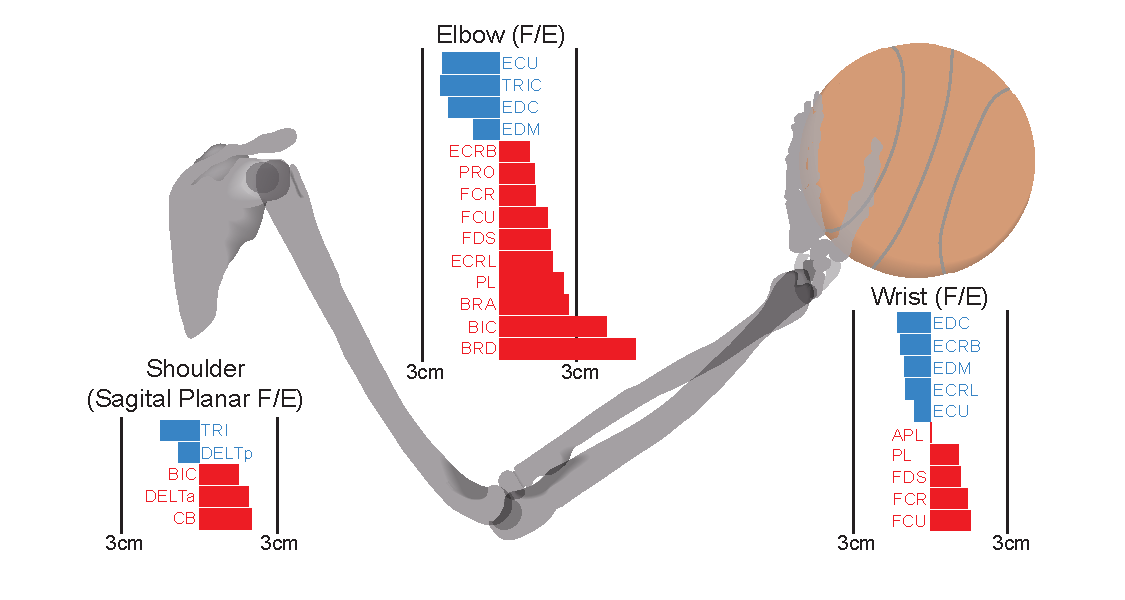
\includegraphics{images/ArmSkeletonFigure}
\caption{18 Muscle, 3 \it dof\rm's Model. Model considers Planar Shoulder Rotation (PSR), Elbow Flexion/Extension (EFE) and Wrist Flexion/Extension (WFE) only. }\label{Figure1}
\end{figure}
\begin{multicols}{2}
\noindent in the ball due to the applied force. The kinematic model was completed using existing literature [4] to incorporate limb lengths as a function of the player’s height, which in turn output the starting position of projectile after a generalized power stroke.\\
Solving the initial value problem based on this ballistic equation provided the instantaneous endpoint velocity vector necessary for a successful attempt based on the position of release. Utilizing an inverse Jacobian matrix generated from the kinematic model, the angular velocities associated with the release posture and the resulting projectile velocity vector were determined: \\
\begin{equation}
\centering \large
\vec{G}( \vec{\theta} )
=
\begin{pmatrix}
G_{x}(\vec{\theta}) \\
G_{y}(\vec{\theta}) \\
G_{\alpha}(\vec{\theta}) \\
\end{pmatrix}
=
\begin{pmatrix}
x \\
y \\
\alpha \\
\end{pmatrix} 
= 
\vec{x}
\end{equation}
\begin{equation}
\centering \large
J = 
\begin{bmatrix}
\frac{\partial G_{x}(\vec{\theta})}{\partial\theta_{1}} & \frac{\partial G_{x}(\vec{\theta})}{\partial\theta_{2}}  & \frac{\partial G_{x}(\vec{\theta})}{\partial\theta_{3}}  \\
\frac{\partial G_{y}(\vec{\theta})}{\partial\theta_{1}} & \frac{\partial G_{y}(\vec{\theta})}{\partial\theta_{2}}  & \frac{\partial G_{y}(\vec{\theta})}{\partial\theta_{3}}  \\
\frac{\partial G_{\alpha}(\vec{\theta})}{\partial\theta_{1}} & \frac{\partial G_{\alpha}(\vec{\theta})}{\partial\theta_{2}}  & \frac{\partial G_{\alpha}(\vec{\theta})}{\partial\theta_{3}}  \\
\end{bmatrix} 
\end{equation}

\begin{equation}
\centering \large
\dot{\vec{x}} = J\dot{\vec{\theta}} \rightarrow \dot{\vec{\theta}} = J^{-1}\dot{\vec{x}}
\end{equation}
Once the final angular velocities were determined we created a program to generate random angular trajectories utilizing cubic spline algorithms and a conservative time course of 550 milliseconds. In order to generate a trajectory this program utilized initial and release angles with corresponding angular velocities as well randomly generated points in configuration space and time within physiologically feasible boundaries. Filters were implemented to account for any undesirable spline algorithm effects. Mainly, we filtered for any trajectories that exhibited angle values outside of the range of motion of a particular joint and we filtered for certain trajectory anomalies not noticed during inspection of a generalized shot attempt (e.g. negative rotation about the shoulder not typical for a generalized shot or sporadic angular acceleration changes in wrist flexion/extension). One hundred thousand random trajectories were generated in total.\\
Utilizing existing literature to construct a posture specific moment arm matrix [1,5,6], it was possible to estimate fiber velocities for each of the 18 muscles considered from the angular velocities generated.
\begin{equation}
\centering
R(\vec{\theta}) 
=
\begin{bmatrix}
r_{1,1}(\vec{\theta}) & r_{1,2}(\vec{\theta}) & \dotsb & r_{1,18}(\vec{\theta}) \\
r_{2,1}(\vec{\theta}) & r_{2,2}(\vec{\theta}) & \dotsb & r_{2,18}(\vec{\theta}) \\
\vdots & \vdots & \ddots & \vdots \\
r_{18,1}(\vec{\theta}) & r_{18,2}(\vec{\theta}) & \dotsb & r_{18,18}(\vec{\theta}) \\
\end{bmatrix}
\end{equation}
\begin{equation}
\centering \large
\delta\vec{s}
=
-R^{T}\delta\vec{\theta}
\end{equation}
\begin{equation}
\centering \large
\vec{v_{m}} \approx \dot{\vec{s}}
=
-R^{T}\dot{\vec{\theta}}
\end{equation}
Assuming stiff tendons we can estimate muscle fiber velocities as the tendon excursion time derivative. Therefore, for each trajectory, a velocity profile was generated for each of the 18 muscles considered (Figure 2). 
\begin{figure}[H]
\centering
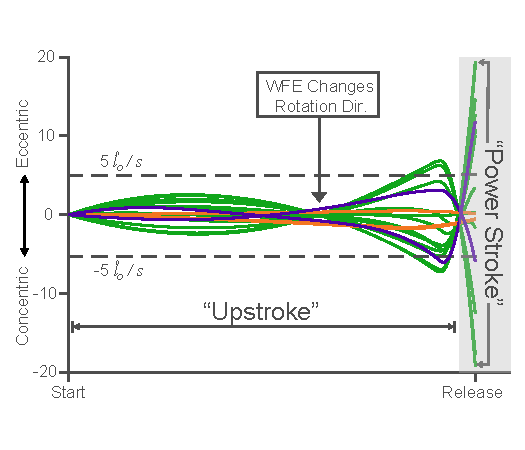
\includegraphics{images/NormalizedMuscleVelocitiesExample}
\caption{Normalized muscle velocities vs. time for a typical free throw attempt.}\label{Figure2}
\end{figure}
\noindent Note that there exists two major zeros crossings within a generalized throw where many of the muscles change the direction of there contractions. The first instance occurs during the upstroke where the wrist and elbow typically remain in a constant posture as the shoulder continues to rotate upwards. The second instance is seen at the start of the power stroke phase where the direction of the elbow and wrist angle rotations change. Note that the muscles that only cross the shoulder (orange) do not cross over the zero velocity line as they typically experience contraction throughout the entire trajectory without a change in direction (i.e. constant upward movement about the shoulder joint). Similarly, as the Biceps and Triceps muscles (purple) cross over both the shoulder and elbow joints, they experience a different zero crossing during the upstroke phase as the shoulder experiences nonzero contraction velocities during this phase. However, they do have typical zero crossings at the start of power stroke phase brought on by a major change in the direction of elbow rotation. Muscles that do not cross over the shoulder at all are shown in green in Figure 2.\\ 
We then classified each trajectory by the magnitudes of the sum of squares of the maximal eccentric and concentric velocities incurred by each muscle throughout the first 520 milliseconds of the movement. As each trial exhibited typically large velocity values both eccentrically and concentrically during the final 30 milliseconds of the power stroke phase, we restricted our classification to the first 520 milliseconds.  
\section*{\normalsize RESULTS}
From the color map in $\textit{Fig. 4 (Bottom)}$ it can be seen that there exists a wide range of shots that are capable of accomplishing the release velocity of a desired throw. More importantly, they can vary greatly in the underlying eccentric and concentric muscle velocities that accompany them, ($\textit{Fig. 3}$). When sampling from these populations, there are multiple cases where kinematically similar basketball free throws have surprisingly different muscle contraction velocity profiles (see cases 1, 2, and 3 in $\textit{Figs. 3 and 4}$). These results explain why a “good looking” shot may, in fact, be fundamentally different from a “good” shot. Moreover, coaching or mimicking the arm trajectory in a way that does not also reveal underlying differences in muscle fiber velocities may explain why a consistently accurate throw is, apparently, so hard to teach, acquire and perfect.
\section*{\normalsize DISCUSSION}
 
\end{multicols}
\begin{figure}[H]
\centering
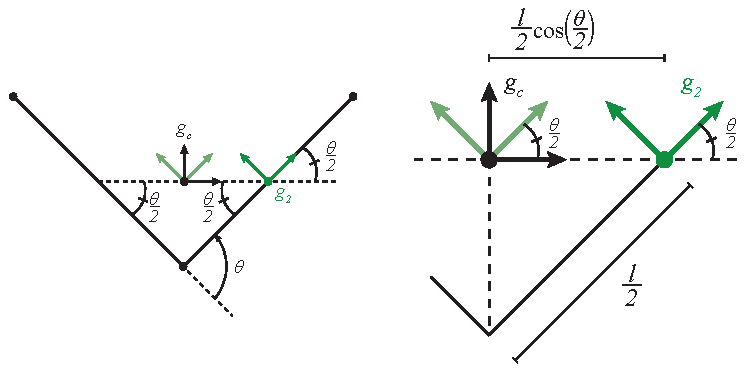
\includegraphics{images/Figure2}
\caption{Three different throw attempts in endpoint space (top) with their corresponding normalized muscle velocity profiles (bottom). Note that the dotted lines in the bottom plots indicate $\pm$ 5  $\hat{l_{o}}/s$.}\label{Figure3}
\end{figure}
\begin{multicols}{2}
\section*{\normalsize CONCLUSION}
Future research will explore the interplay between these strong kinematic constraints, and the neuromechanical regulation, timing and coordination of alpha-gamma co-activation, muscle excitation$\backslash$contraction dynamics, motor unit recruitment, signal-dependent noise, and neural conduction delays.
\section*{\normalsize REFERENCES}
\begin{flushleft}
1. Valero-Cuevas, FJ, \it Fundamentals of Neuromechanics\rm, Springer-Verlag London, 2016. \break
2. Valero-Cuevas, F, Cohn, B, Yngvason, H, $\&$ Lawrence, E, \it J Biomech\rm,  $\textbf{48}$(11), 2887-2896, 2015. \break
3. Sherrington, C.S. \it Exp. Physiol.\rm, $\textbf{6}$(3) 252-310, 1913. \break
4. Winter, DA, \it Biomechanics and motor control of human movement: Fourth edition \rm, Elsevier B.V., 2013.\linebreak
5. Ramsay, JW, Hunter, BV, $\&$ Gonzalez, RV, \it J Biomech\rm, $\textbf{42}$(4), 463-473, 2009. \break
6. Holzbaur, KR, Murray, WM, $\&$ Delp, SL, \it Annals of Biomedical Engineering\rm, $\textbf{33}$(6), 829-840, 2005.
\end{flushleft}
\section*{\normalsize ACKNOWLEDGEMENTS}
We thank the University of Southern California for facilities provided during the course BME/BKN 504, Brian Cohn for his help with the illustrations, and Emily Lawrence who laid the foundation for this research and shared her prior work.
\end{multicols}
\begin{figure}[H]
\centering
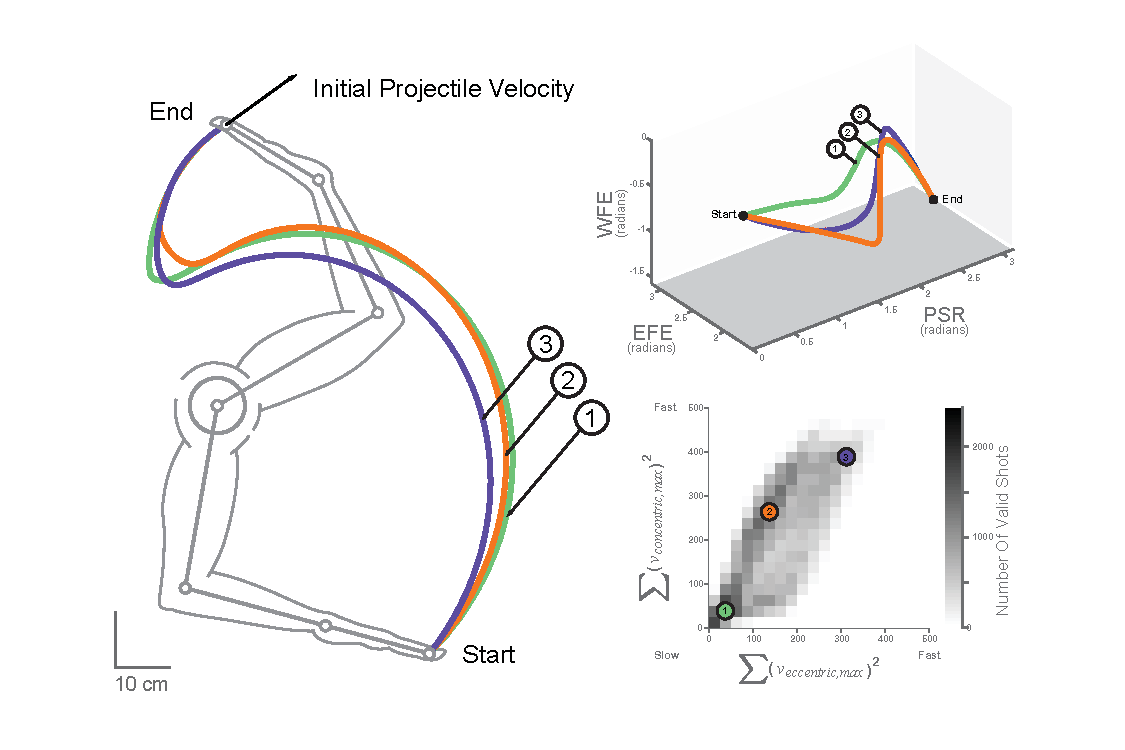
\includegraphics{images/Figure3}
\caption{2D Histogram (Bottom) of 10k Shots with Trials 1, 2 and 3 plotted in Configuration Space (Middle) and Endpoint Space (Top).}\label{Figure4}
\end{figure}
\end{document}